\documentclass[
11pt, % The default document font size, options: 10pt, 11pt, 12pt
%codirector, % Uncomment to add a codirector to the title page
]{charter} 




% El títulos de la memoria, se usa en la carátula y se puede usar el cualquier lugar del documento con el comando \ttitle
\titulo{Sistema de monitoreo de ocupación en
espacios internos mediante BLE \textit{Beacons}} 

% Nombre del posgrado, se usa en la carátula y se puede usar el cualquier lugar del documento con el comando \degreename
%\posgrado{Carrera de Especialización en Sistemas Embebidos} 
\posgrado{Carrera de Especialización en Internet de las Cosas} 
%\posgrado{Carrera de Especialización en Intelegencia Artificial}
%\posgrado{Maestría en Sistemas Embebidos} 
%\posgrado{Maestría en Internet de las cosas}

% Tu nombre, se puede usar el cualquier lugar del documento con el comando \authorname
\autor{Ing. Facundo Fernández} 

% El nombre del director y co-director, se puede usar el cualquier lugar del documento con el comando \supname y \cosupname y \pertesupname y \pertecosupname
\director{Nombre del Director}
\pertenenciaDirector{pertenencia} 
% FIXME:NO IMPLEMENTADO EL CODIRECTOR ni su pertenencia
\codirector{John Doe} % para que aparezca en la portada se debe descomentar la opción codirector en el documentclass
\pertenenciaCoDirector{FIUBA}

% Nombre del cliente, quien va a aprobar los resultados del proyecto, se puede usar con el comando \clientename y \empclientename
\cliente{Nombre del cliente}
\empresaCliente{Empresa del cliente}

% Nombre y pertenencia de los jurados, se pueden usar el cualquier lugar del documento con el comando \jurunoname, \jurdosname y \jurtresname y \perteunoname, \pertedosname y \pertetresname.
\juradoUno{Nombre y Apellido (1)}
\pertenenciaJurUno{pertenencia (1)} 
\juradoDos{Nombre y Apellido (2)}
\pertenenciaJurDos{pertenencia (2)}
\juradoTres{Nombre y Apellido (3)}
\pertenenciaJurTres{pertenencia (3)}
 
\fechaINICIO{17 de octubre de 2023}		%Fecha de inicio de la cursada de GdP \fechaInicioName
\fechaFINALPlan{05 de diciembre de 2023} 	%Fecha de final de cursada de GdP
\fechaFINALTrabajo{15 de junio de 2024}	%Fecha de defensa pública del trabajo final


\begin{document}

\maketitle
\thispagestyle{empty}
\pagebreak


\thispagestyle{empty}
{\setlength{\parskip}{0pt}
\tableofcontents{}
}
\pagebreak


\section*{Registros de cambios}
\label{sec:registro}


\begin{table}[ht]
\label{tab:registro}
\centering
\begin{tabularx}{\linewidth}{@{}|c|X|c|@{}}
\hline
\rowcolor[HTML]{C0C0C0} 
Revisión & \multicolumn{1}{c|}{\cellcolor[HTML]{C0C0C0}Detalles de los cambios realizados} & Fecha      \\ \hline
0      & Creación del documento                                 &\fechaInicioName \\ \hline
1      & Se completa hasta el punto 5 inclusive                 & 31 de octubre de 2023 \\ \hline
%2      & Se completa hasta el punto 9 inclusive
%		  Se puede agregar algo más \newline
%		  En distintas líneas \newline
%		  Así                                                    & dd/mm/aaaa \\ \hline
%3      & Se completa hasta el punto 11 inclusive                & dd/mm/aaaa \\ \hline
%4      & Se completa el plan	                                 & dd/mm/aaaa \\ \hline
\end{tabularx}
\end{table}

\pagebreak



\section*{Acta de constitución del proyecto}
\label{sec:acta}

\begin{flushright}
Buenos Aires, \fechaInicioName
\end{flushright}

\vspace{2cm}

Por medio de la presente se acuerda con el Ing. \authorname\hspace{1px} que su Trabajo Final de la \degreename\hspace{1px} se titulará ``\ttitle'', consistirá esencialmente en la implementación de un prototipo de un sistema de monitoreo de ocupación utilizando \textit{Beacons Bluetooth Low Energy}, y tendrá un presupuesto preliminar estimado de {600} h de trabajo y {\$200} USD, con fecha de inicio \fechaInicioName\hspace{1px} y fecha de presentación pública \fechaFinalName.

Se adjunta a esta acta la planificación inicial.

\vfill

% Esta parte se construye sola con la información que hayan cargado en el preámbulo del documento y no debe modificarla
\begin{table}[ht]
\centering
\begin{tabular}{ccc}
\begin{tabular}[c]{@{}c@{}}Dr. Ing. Ariel Lutenberg \\ Director posgrado FIUBA\end{tabular} & \hspace{2cm} & \begin{tabular}[c]{@{}c@{}}\clientename \\ \empclientename \end{tabular} \vspace{2.5cm} \\ 
\multicolumn{3}{c}{\begin{tabular}[c]{@{}c@{}} \supname \\ Director del Trabajo Final\end{tabular}} \vspace{2.5cm} \\
%\begin{tabular}[c]{@{}c@{}}\jurunoname \\ Jurado del Trabajo Final\end{tabular}     &  & \begin{tabular}[c]{@{}c@{}}\jurdosname\\ Jurado del Trabajo Final\end{tabular}  \vspace{2.5cm}  \\
%\multicolumn{3}{c}{\begin{tabular}[c]{@{}c@{}} \jurtresname\\ Jurado del Trabajo Final\end{tabular}} \vspace{.5cm}                                                                     
\end{tabular}
\end{table}




\section{1. Descripción técnica-conceptual del proyecto a realizar}
\label{sec:descripcion}

El proyecto nace como un emprendimiento personal con un enfoque específico para gimnasios y recintos deportivos en donde los usuarios (clientes del gimnasio) pueden acceder a distintas horas sin ningún tipo de limitación. Este emprendimiento surge de la necesidad de entender el comportamiento de usuarios en gimnasios con el objetivo de proporcionar al cliente (propietario del gimnasio) la capacidad de entender a su clientela y cómo usan sus instalaciones. 

Adicional, esta herramienta permite entender el tiempo de visita de una persona. El tiempo de visita es una medida sumamente importante para entender a los usuarios que se mantienen como clientes de un gimnasio y a los que no. En el contexto de clientes de gimnasios, es más económico retener a una persona para que siga siendo cliente que conseguir nuevos. El objetivo general es poder dar una herramienta más a los gimnasios donde puedan utilizar datos para tomar decisiones de negocio.

Debido a que este proyecto es un prototipo y un emprendimiento personal, no se cuenta con financiamiento de ningún tipo, por lo que se trabajará en diseñar un sistema funcional que cumpla con las características de un mínimo producto viable, financiado completamente por el autor de este documento. Una de las ventajas de abordarlo de esta manera es que no existen limitaciones de desarrollo ni hay ningún interesado que pueda tener incidencia en el resultado final del trabajo.

En el contexto actual de la tecnología y la creciente demanda de soluciones de posicionamiento en interiores, el presente proyecto se centra en la implementación de un sistema innovador de monitoreo de ocupación en espacios interiores utilizando la tecnología \textit{Bluetooth Low Energy} (BLE) \textit{Beacons}. Esta tecnología permite la ubicación precisa de dispositivos móviles en entornos cerrados, brindando a los usuarios una experiencia de ubicación confiable y en tiempo real. 

La esencia de este proyecto radica en proporcionar a los propietarios de recintos o edificios una herramienta para la gestión eficiente de la ocupación, así como una herramienta más de recaudación de datos de uso y comportamiento. La solución propuesta se distingue por su capacidad para ofrecer datos precisos y actualizados sobre la cantidad de personas presentes en el recinto en cualquier momento dado, así como la capacidad de determinar el tiempo de visita promedio de un usuario.

El desafío que aborda este proyecto es la falta de sistemas de monitoreo de ocupación precisos y en tiempo real en entornos interiores. La tecnología BLE \textit{Beacons} junto con la estación base ESP32-C3 proporciona una solución efectiva y rentable. Mediante la emisión de señales de baja energía, los \textit{Beacons} identifican la presencia de dispositivos móviles, permitiendo a la aplicación de monitoreo determinar la ocupación actual a través de un algoritmo de triangulación. Esta información se almacena en una base de datos no relacional alojada en MongoDB, brindando al propietario acceso a datos cruciales para la toma de decisiones informadas.

El sistema se compone de cuatro elementos principales: los BLE \textit{Beacons}, la estación base ESP32-C3, la aplicación de monitoreo y la base de datos no relacional. Los \textit{Beacons} emiten señales identificativas, que son escaneadas por la estación base. La aplicación de monitoreo procesa estas señales para determinar la proximidad de los dispositivos móviles y actualiza la base de datos con la información de ocupación. A través de un panel de control intuitivo, el propietario del recinto puede visualizar la ocupación actual y acceder a informes históricos. En la Figura \ref{fig:diagBloques} se presenta el diagrama de bloques del sistema, donde se observa claramente la distribución y diseño de los componentes clave.

\begin{figure}[htpb]
\centering 
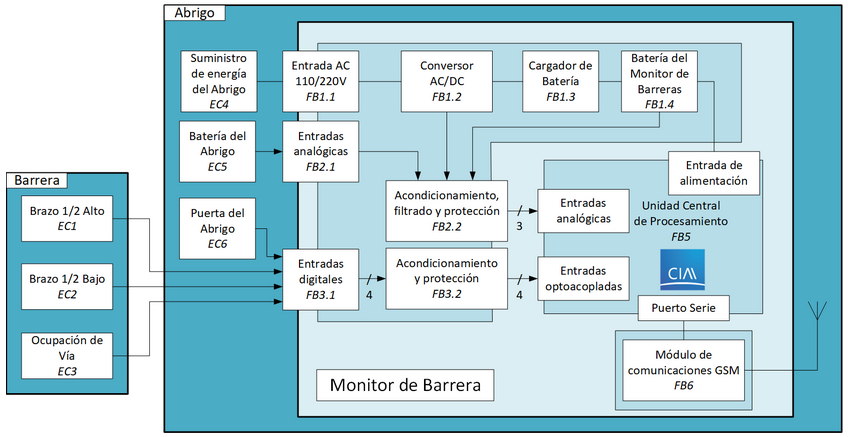
\includegraphics[width=.7\textwidth]{./Figuras/diagBloques.png}
\caption{Diagrama en bloques del sistema.}
\label{fig:diagBloques}
\end{figure}

\vspace{25px}

La innovación radica en la combinación efectiva de la tecnología BLE \textit{Beacons} con la estación base ESP32-C3 para ofrecer una solución escalable y rentable de monitoreo de ocupación en interiores. Esta solución se destaca por su capacidad para proporcionar datos precisos y accesibles, sentando las bases para futuras implementaciones en diversos entornos comerciales y públicos. 

Para la realización de este trabajo, se probarán y utilizarán hasta 6 \textit{beacons} o balizas en un entorno reducido, con el objetivo de probar la viabilidad del proyecto. Este entorno reducido no superará los 50 m$^2$ y será en un ambiente doméstico. Para el panel de control se creará una aplicación accesible sólo a través de web, con el objetivo de reducir costos de desarrollo.

\section{2. Identificación y análisis de los interesados}
\label{sec:interesados}

Dado que este proyecto es de carácter personal, no involucra a interesados externos o a un equipo de trabajo formal. En este contexto, la principal parte interesada es el autor, como el iniciador y ejecutor del proyecto. Como único responsable, el autor asume todas las funciones, desde la planificación y desarrollo hasta la gestión económica y control de entregables. Esta autonomía proporciona flexibilidad y agilidad en la toma de decisiones, permitiendo una ejecución eficiente del proyecto.

En calidad de responsable, el rol abarca la supervisión integral del proyecto, incluyendo la gestión económica, planificación de tareas, desarrollo de los componentes técnicos y aseguramiento de la calidad de los entregables. Además, el responsable asume la responsabilidad de mantener el proyecto dentro de los plazos establecidos y gestionar eficazmente los recursos disponibles.

El director, por su parte, desempeñará un papel esencial al brindar orientación y asesoramiento experto en todas las facetas del proyecto. Se espera que actúe como un referente en cuestiones técnicas y organizativas desde el inicio hasta la finalización del proyecto, aportando valiosos conocimientos y experiencia para asegurar su éxito. Su apoyo será fundamental para superar cualquier desafío que pueda surgir a lo largo del desarrollo del proyecto.

\begin{table}[ht]
%\caption{Identificación de los interesados}
%\label{tab:interesados}
\begin{tabularx}{\linewidth}{@{}|l|X|X|l|@{}}
\hline
\rowcolor[HTML]{C0C0C0} 
Rol           & Nombre y Apellido & Organización 	& Puesto 	\\ \hline
Cliente       & \clientename      &\empclientename	&        	\\ \hline
Responsable   & \authorname       & FIUBA        	& Alumno 	\\ \hline
Orientador    & \supname	      & \pertesupname 	& Director Trabajo final \\ \hline
\end{tabularx}
\end{table}



\section{3. Propósito del proyecto}
\label{sec:proposito}

El propósito de este proyecto es implementar un sistema de monitoreo de ocupación en espacios interiores, principalmente en gimnasios, mediante la tecnología \textit{Bluetooth Low Energy} (BLE) \textit{Beacons}. Se busca proporcionar al propietario del recinto datos precisos, históricos y de calidad sobre la cantidad de personas presentes en cualquier momento dado, permitiendo así una gestión eficiente de la ocupación y una toma de decisiones informadas a través de datos con el objetivo de medir el comportamiento de los usuarios. Esta solución pionera sienta las bases para futuras implementaciones en diversos entornos comerciales y públicos, abriendo nuevas posibilidades en el campo del posicionamiento en interiores.

\section{4. Alcance del proyecto}
\label{sec:alcance}

El presente proyecto incluye:
\begin{itemize}
	\item La planificación, diseño, implementación y puesta en funcionamiento de un sistema de monitoreo de ocupación en espacios interiores utilizando la tecnología \textit{Bluetooth Low Energy} (BLE) \textit{Beacons} en un espacio no mayor a los 50 m$^2$.
	\item La adquisición y ubicación estratégica de los BLE \textit{Beacons}, así como la configuración de la estación base ESP32-C3 y el desarrollo de la aplicación web de monitoreo. 
	\item La implementación de una base de datos no relacional en MongoDB para el almacenamiento y gestión de la información de ocupación. 
	\item Pruebas para verificar el funcionamiento correcto del sistema 
	\item Una interfaz de usuario intuitiva en forma de panel de control para que el propietario del recinto pueda visualizar la ocupación actual, acceder a informes históricos y analizar los datos si lo considera necesario.
	\item La cobertura de todos los costos relacionados con el desarrollo, como son el hardware y software por parte del autor.
\end{itemize}


El presente proyecto no incluye:
\begin{itemize}
	\item La adquisición de hardware o software adicional no especificado en los requerimientos, salvo que sea necesario para la integración del sistema y se determine previamente.
	\item La adquisición o configuración de servicios de conectividad de red, como proveedores de internet o servicios de datos móviles.
	\item Mantenimiento continuo del sistema después de la finalización del proyecto.
	\item La capacitación avanzada en programación o configuración de hardware que no esté directamente relacionada con el sistema implementado.
	\item Una aplicación de configuración del sistema, a menos que el autor lo requiera.
\end{itemize}

Cualquier modificación o extensión del alcance del proyecto requerirá una revisión y aprobación previa por parte del director del proyecto y el responsable de este.


\section{5. Supuestos del proyecto}
\label{sec:supuestos}

Para el desarrollo del presente proyecto se supone que:

\begin{itemize}
	\item Disponibilidad de recursos humanos: se asume que el responsable del proyecto contará con el tiempo y dedicación necesarios para llevar a cabo todas las etapas de planificación, implementación y puesta en marcha del sistema. Además, se presupone la colaboración activa del director para brindar orientación técnica y organizativa.
	\item Estabilidad de las condiciones del entorno: se supone que las condiciones ambientales y estructurales en los recintos seleccionados serán estables y no experimentarán cambios significativos durante el período de implementación del proyecto. Por condiciones ambientales y estructurales se refiere a la disposición física del espacio como paredes y muebles, así como fluctuaciones significativas en la temperatura o en la humedad ya que estas pueden influir en cómo las señales \textit{Bluetooth} se propagan en el espacio.
	\item Disponibilidad de equipamiento y materiales: se presupone que se podrá adquirir el hardware necesario, incluyendo los BLE \textit{Beacons} y la estación base ESP32-C3, así como cualquier otro equipo o material requerido para la implementación del sistema.
	\item Presupuesto: se supone que el presupuesto establecido de {\$200} USD será suficiente para cubrir los costos de hardware y software, así como cualquier otro material requerido para la implementación del sistema. En caso de incurrir en un gasto mayor, se evaluará la viabilidad, manteniendo un tope máximo de {\$1,000} USD.
	\item Factibilidad técnica: se considera que la tecnología BLE \textit{Beacons} y el microcontrolador ESP32-C3 son adecuados para la aplicación prevista y no presentarán inconvenientes técnicos significativos en su configuración y funcionamiento.
	\item Cumplimiento de regulaciones y normativas: se parte del supuesto de que el proyecto cumple con todas las regulaciones y normativas locales, estatales y federales aplicables y que no se requerirá de permisos o licencias adicionales para la implementación del sistema.
	\item Estabilidad de los protocolos de comunicación: se presupone que los protocolos de Internet estándar seleccionados (HTTP o MQTT) para la comunicación entre la aplicación móvil y la base de datos funcionarán de manera estable y confiable.
	\item Acceso a la tecnología y herramientas: se asume que se contará con acceso a las tecnologías y herramientas necesarias para el desarrollo de la aplicación de monitoreo y la configuración de la base de datos en MongoDB.
	\item Disponibilidad de energía eléctrica: se presupone que se dispondrá de suministro eléctrico confiable ya sea a través de baterías o red eléctrica para alimentar tanto los BLE \textit{Beacons} como la estación base y demás equipos asociados al sistema.
	\item Compatibilidad de dispositivos móviles: se supone que los dispositivos móviles que se encuentren en el rango de los BLE \textit{Beacons} serán compatibles con la tecnología \textit{Bluetooth Low Energy} y podrán recibir las señales emitidas. 
\end{itemize}

\section{6. Requerimientos}
\label{sec:requerimientos}

\begin{consigna}{red}
Los requerimientos deben numerarse y de ser posible estar agruparlos por afinidad, por ejemplo:

\begin{enumerate}
	\item Requerimientos funcionales
		\begin{enumerate}
			\item El sistema debe...
			\item Tal componente debe...
			\item El usuario debe poder...
		\end{enumerate}
	\item Requerimientos de documentación
		\begin{enumerate}
			\item Requerimiento 1
			\item Requerimiento 2 (prioridad menor)
		\end{enumerate}
	\item Requerimiento de testing...
	\item Requerimientos de la interfaz...
	\item Requerimientos interoperabilidad...
	\item etc...
\end{enumerate}

Leyendo los requerimientos se debe poder interpretar cómo será el proyecto y su funcionalidad.

Indicar claramente cuál es la prioridad entre los distintos requerimientos y si hay requerimientos opcionales. 

No olvidarse de que los requerimientos incluyen a las regulaciones y normas vigentes!!!

Y al escribirlos seguir las siguientes reglas:
\begin{itemize}
	\item Ser breve y conciso (nadie lee cosas largas). 
	\item Ser específico: no dejar lugar a confusiones.
	\item Expresar los requerimientos en términos que sean cuantificables y medibles.
\end{itemize}

\end{consigna}

\section{7. Historias de usuarios (\textit{Product backlog})}
\label{sec:backlog}

\begin{consigna}{red}
Descripción: En esta sección se deben incluir las historias de usuarios y su ponderación (\textit{history points}). Recordar que las historias de usuarios son descripciones cortas y simples de una característica contada desde la perspectiva de la persona que desea la nueva capacidad, generalmente un usuario o cliente del sistema. La ponderación es un número entero que representa el tamaño de la historia comparada con otras historias de similar tipo.

El formato propuesto es: "como [rol] quiero [tal cosa] para [tal otra cosa]."

Se debe indicar explícitamente el criterio para calcular los \textit{story points} de cada historia
\end{consigna}

\section{8. Entregables principales del proyecto}
\label{sec:entregables}

\begin{consigna}{red}

Los entregables del proyecto son (ejemplo):

\begin{itemize}
	\item Manual de uso
	\item Diagrama de circuitos esquemáticos
	\item Código fuente del firmware
	\item Diagrama de instalación
	\item Informe final
	\item etc...
\end{itemize}

\end{consigna}

\section{9. Desglose del trabajo en tareas}
\label{sec:wbs}

\begin{consigna}{red}
El WBS debe tener relación directa o indirecta con los requerimientos.  Son todas las actividades que se harán en el proyecto para dar cumplimiento a los requerimientos. Se recomienda mostrar el WBS mediante una lista indexada:

\begin{enumerate}
\item Grupo de tareas 1
	\begin{enumerate}
	\item Tarea 1 (tantas h)
	\item Tarea 2 (tantas hs)
	\item Tarea 3 (tantas h)
	\end{enumerate}
\item Grupo de tareas 2
	\begin{enumerate}
	\item Tarea 1 (tantas h)
	\item Tarea 2 (tantas h)
	\item Tarea 3 (tantas h)
	\end{enumerate}
\item Grupo de tareas 3
	\begin{enumerate}
	\item Tarea 1 (tantas h)
	\item Tarea 2 (tantas h)
	\item Tarea 3 (tantas h)
	\item Tarea 4 (tantas h)
	\item Tarea 5 (tantas h)
	\end{enumerate}
\end{enumerate}

Cantidad total de horas: (tantas h)

Se recomienda que no haya ninguna tarea que lleve más de 40 h. 

\end{consigna}

\section{10. Diagrama de Activity On Node}
\label{sec:AoN}

\begin{consigna}{red}
Armar el AoN a partir del WBS definido en la etapa anterior. 

%La figura \ref{fig:AoN} fue elaborada con el paquete latex tikz y pueden consultar la siguiente referencia \textit{online}:

%\url{https://www.overleaf.com/learn/latex/LaTeX_Graphics_using_TikZ:_A_Tutorial_for_Beginners_(Part_3)\%E2\%80\%94Creating_Flowcharts}

\end{consigna}

\begin{figure}[htpb]
\centering 
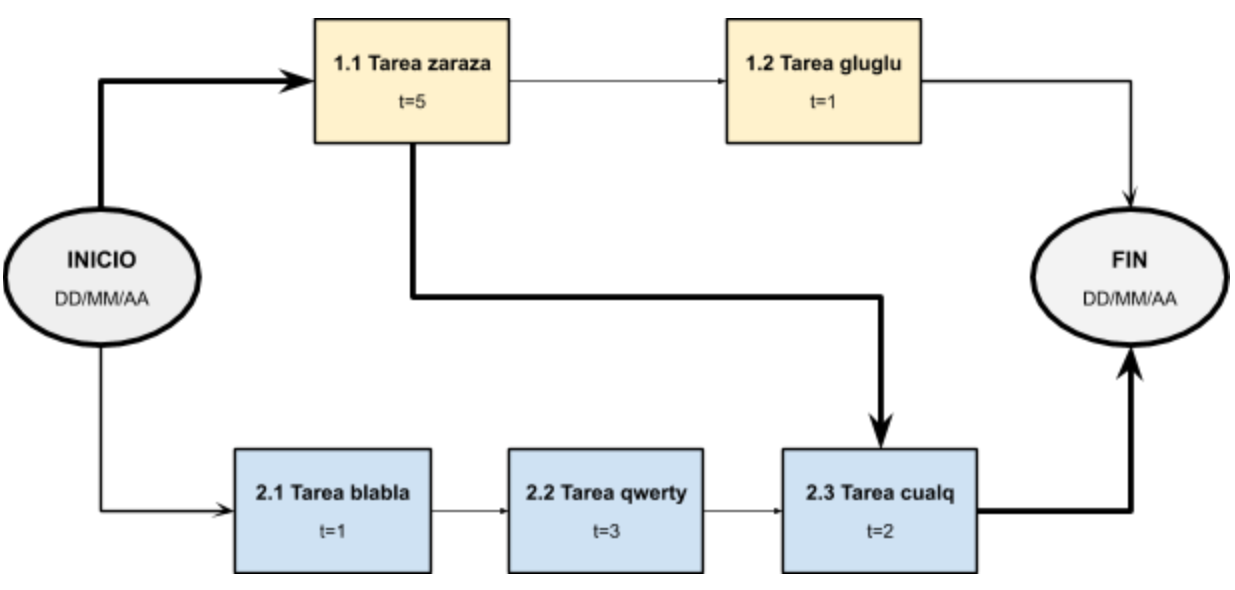
\includegraphics[width=.8\textwidth]{./Figuras/AoN.png}
\caption{Diagrama de \textit{Activity on Node}.}
\label{fig:AoN}
\end{figure}

Indicar claramente en qué unidades están expresados los tiempos.
De ser necesario indicar los caminos semicríticos y analizar sus tiempos mediante un cuadro.
Es recomendable usar colores y un cuadro indicativo describiendo qué representa cada color, como se muestra en el siguiente ejemplo:



\section{11. Diagrama de Gantt}
\label{sec:gantt}

\begin{consigna}{red}

Existen muchos programas y recursos \textit{online} para hacer diagramas de Gantt, entre los cuales destacamos:

\begin{itemize}
\item Planner
\item GanttProject
\item Trello + \textit{plugins}. En el siguiente link hay un tutorial oficial: \\ \url{https://blog.trello.com/es/diagrama-de-gantt-de-un-proyecto}
\item Creately, herramienta online colaborativa. \\\url{https://creately.com/diagram/example/ieb3p3ml/LaTeX}
\item Se puede hacer en latex con el paquete \textit{pgfgantt}\\ \url{http://ctan.dcc.uchile.cl/graphics/pgf/contrib/pgfgantt/pgfgantt.pdf}
\end{itemize}

Pegar acá una captura de pantalla del diagrama de Gantt, cuidando que la letra sea suficientemente grande como para ser legible. 
Si el diagrama queda demasiado ancho, se puede pegar primero la ``tabla'' del Gantt y luego pegar la parte del diagrama de barras del diagrama de Gantt.

Configurar el software para que en la parte de la tabla muestre los códigos del EDT (WBS).\\
Configurar el software para que al lado de cada barra muestre el nombre de cada tarea.\\
Revisar que la fecha de finalización coincida con lo indicado en el Acta Constitutiva.

En la figura \ref{fig:gantt}, se muestra un ejemplo de diagrama de Gantt realizado con el paquete de \textit{pgfgantt}. En la plantilla pueden ver el código que lo genera y usarlo de base para construir el propio.

\begin{figure}[htbp]
\begin{center}
\begin{ganttchart}{1}{12}
  \gantttitle{2020}{12} \\
  \gantttitlelist{1,...,12}{1} \\
  \ganttgroup{Group 1}{1}{7} \\
  \ganttbar{Task 1}{1}{2} \\
  \ganttlinkedbar{Task 2}{3}{7} \ganttnewline
  \ganttmilestone{Milestone o hito}{7} \ganttnewline
  \ganttbar{Final Task}{8}{12}
  \ganttlink{elem2}{elem3}
  \ganttlink{elem3}{elem4}
\end{ganttchart}
\end{center}
\caption{Diagrama de Gantt de ejemplo}
\label{fig:gantt}
\end{figure}


\begin{landscape}
\begin{figure}[htpb]
\centering 
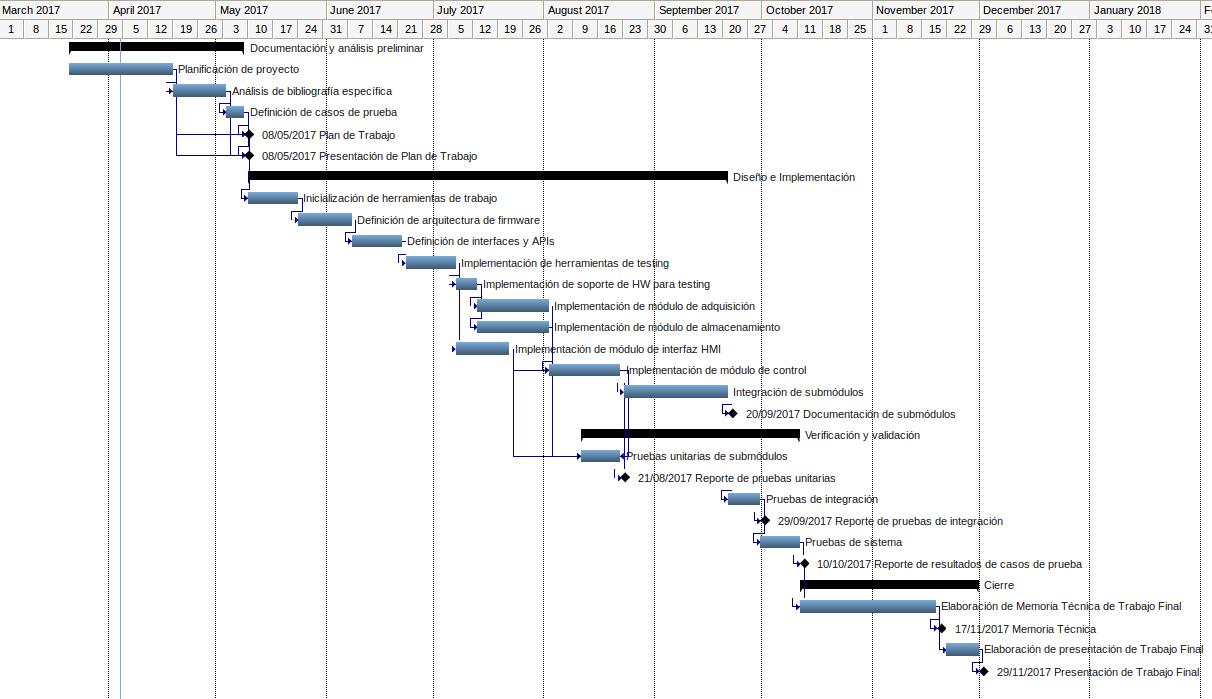
\includegraphics[height=.85\textheight]{./Figuras/Gantt-2.png}
\caption{Ejemplo de diagrama de Gantt rotado}
\label{fig:diagGantt}
\end{figure}

\end{landscape}

\end{consigna}


\section{12. Presupuesto detallado del proyecto}
\label{sec:presupuesto}

\begin{consigna}{red}
Si el proyecto es complejo entonces separarlo en partes:
\begin{itemize}
	\item Un total global, indicando el subtotal acumulado por cada una de las áreas.
	\item El desglose detallado del subtotal de cada una de las áreas.
\end{itemize}

IMPORTANTE: No olvidarse de considerar los COSTOS INDIRECTOS.

\end{consigna}

\begin{table}[htpb]
\centering
\begin{tabularx}{\linewidth}{@{}|X|c|r|r|@{}}
\hline
\rowcolor[HTML]{C0C0C0} 
\multicolumn{4}{|c|}{\cellcolor[HTML]{C0C0C0}COSTOS DIRECTOS} \\ \hline
\rowcolor[HTML]{C0C0C0} 
Descripción &
  \multicolumn{1}{c|}{\cellcolor[HTML]{C0C0C0}Cantidad} &
  \multicolumn{1}{c|}{\cellcolor[HTML]{C0C0C0}Valor unitario} &
  \multicolumn{1}{c|}{\cellcolor[HTML]{C0C0C0}Valor total} \\ \hline
 &
  \multicolumn{1}{c|}{} &
  \multicolumn{1}{c|}{} &
  \multicolumn{1}{c|}{} \\ \hline
 &
  \multicolumn{1}{c|}{} &
  \multicolumn{1}{c|}{} &
  \multicolumn{1}{c|}{} \\ \hline
\multicolumn{1}{|l|}{} &
   &
   &
   \\ \hline
\multicolumn{1}{|l|}{} &
   &
   &
   \\ \hline
\multicolumn{3}{|c|}{SUBTOTAL} &
  \multicolumn{1}{c|}{} \\ \hline
\rowcolor[HTML]{C0C0C0} 
\multicolumn{4}{|c|}{\cellcolor[HTML]{C0C0C0}COSTOS INDIRECTOS} \\ \hline
\rowcolor[HTML]{C0C0C0} 
Descripción &
  \multicolumn{1}{c|}{\cellcolor[HTML]{C0C0C0}Cantidad} &
  \multicolumn{1}{c|}{\cellcolor[HTML]{C0C0C0}Valor unitario} &
  \multicolumn{1}{c|}{\cellcolor[HTML]{C0C0C0}Valor total} \\ \hline
\multicolumn{1}{|l|}{} &
   &
   &
   \\ \hline
\multicolumn{1}{|l|}{} &
   &
   &
   \\ \hline
\multicolumn{1}{|l|}{} &
   &
   &
   \\ \hline
\multicolumn{3}{|c|}{SUBTOTAL} &
  \multicolumn{1}{c|}{} \\ \hline
\rowcolor[HTML]{C0C0C0}
\multicolumn{3}{|c|}{TOTAL} &
   \\ \hline
\end{tabularx}%
\end{table}


\section{13. Gestión de riesgos}
\label{sec:riesgos}

\begin{consigna}{red}
a) Identificación de los riesgos (al menos cinco) y estimación de sus consecuencias:
 
Riesgo 1: detallar el riesgo (riesgo es algo que si ocurre altera los planes previstos de forma negativa)
\begin{itemize}
	\item Severidad (S): mientras más severo, más alto es el número (usar números del 1 al 10).\\
	Justificar el motivo por el cual se asigna determinado número de severidad (S).
	\item Probabilidad de ocurrencia (O): mientras más probable, más alto es el número (usar del 1 al 10).\\
	Justificar el motivo por el cual se asigna determinado número de (O). 
\end{itemize}   

Riesgo 2:
\begin{itemize}
	\item Severidad (S): 
	\item Ocurrencia (O):
\end{itemize}

Riesgo 3:
\begin{itemize}
	\item Severidad (S): 
	\item Ocurrencia (O):
\end{itemize}


b) Tabla de gestión de riesgos:      (El RPN se calcula como RPN=SxO)

\begin{table}[htpb]
\centering
\begin{tabularx}{\linewidth}{@{}|X|c|c|c|c|c|c|@{}}
\hline
\rowcolor[HTML]{C0C0C0} 
Riesgo & S & O & RPN & S* & O* & RPN* \\ \hline
       &   &   &     &    &    &      \\ \hline
       &   &   &     &    &    &      \\ \hline
       &   &   &     &    &    &      \\ \hline
       &   &   &     &    &    &      \\ \hline
       &   &   &     &    &    &      \\ \hline
\end{tabularx}%
\end{table}

Criterio adoptado: 
Se tomarán medidas de mitigación en los riesgos cuyos números de RPN sean mayores a...

Nota: los valores marcados con (*) en la tabla corresponden luego de haber aplicado la mitigación.

c) Plan de mitigación de los riesgos que originalmente excedían el RPN máximo establecido:
 
Riesgo 1: plan de mitigación (si por el RPN fuera necesario elaborar un plan de mitigación).
  Nueva asignación de S y O, con su respectiva justificación:
  - Severidad (S): mientras más severo, más alto es el número (usar números del 1 al 10).
          Justificar el motivo por el cual se asigna determinado número de severidad (S).
  - Probabilidad de ocurrencia (O): mientras más probable, más alto es el número (usar del 1 al 10).
          Justificar el motivo por el cual se asigna determinado número de (O).

Riesgo 2: plan de mitigación (si por el RPN fuera necesario elaborar un plan de mitigación).
 
Riesgo 3: plan de mitigación (si por el RPN fuera necesario elaborar un plan de mitigación).

\end{consigna}


\section{14. Gestión de la calidad}
\label{sec:calidad}

\begin{consigna}{red}
Elija al menos diez requerientos que a su criterio sean los más importantes/críticos/que aportan más valor y para cada uno de ellos indique las acciones de verificación y validación que permitan asegurar su cumplimiento.

\begin{itemize} 
\item Req \#1: copiar acá el requerimiento.

\begin{itemize}
	\item Verificación para confirmar si se cumplió con lo requerido antes de mostrar el sistema al cliente. Detallar 
	\item Validación con el cliente para confirmar que está de acuerdo en que se cumplió con lo requerido. Detallar  
\end{itemize}

\end{itemize}

Tener en cuenta que en este contexto se pueden mencionar simulaciones, cálculos, revisión de hojas de datos, consulta con expertos, mediciones, etc.  Las acciones de verificación suelen considerar al entregable como ``caja blanca'', es decir se conoce en profundidad su funcionamiento interno.  En cambio, las acciones de validación suelen considerar al entregable como ``caja negra'', es decir, que no se conocen los detalles de su funcionamiento interno.

\end{consigna}

\section{15. Procesos de cierre}    
\label{sec:cierre}

\begin{consigna}{red}
Establecer las pautas de trabajo para realizar una reunión final de evaluación del proyecto, tal que contemple las siguientes actividades:

\begin{itemize}
	\item Pautas de trabajo que se seguirán para analizar si se respetó el Plan de Proyecto original:
	 - Indicar quién se ocupará de hacer esto y cuál será el procedimiento a aplicar. 
	\item Identificación de las técnicas y procedimientos útiles e inútiles que se emplearon, y los problemas que surgieron y cómo se solucionaron:
	 - Indicar quién se ocupará de hacer esto y cuál será el procedimiento para dejar registro.
	\item Indicar quién organizará el acto de agradecimiento a todos los interesados, y en especial al equipo de trabajo y colaboradores:
	  - Indicar esto y quién financiará los gastos correspondientes.
\end{itemize}

\end{consigna}


\end{document}
